\Chapter{A Szoftver Megtervezése}

\Section{Koncepció}

Mivel a szakdolgozat egyszerre foglalkozik kutatási és szoftverfejlesztési témákkal, a dolgozat kidolgozása során szükséges a két területtel egyszerre foglalkozni.\\ 

A kutatás alapvetően a \hyperlink{chapter.2}{Node Package Manager (npm)} megismeréséhez, működésének megértéséhez fűződik, míg a fejlesztés egy olyan program megtervezése, amely megfelelően implementálja az npm funkcióit a feladatai elvégzéséhez.

A kutatás másik fontos mérföldköve volt felmérni a \hyperlink{section.3.2}{hasonló programok} meglétét, kivitelezésének formáját. A tapasztalatok alapján érdekes, de alapvető funkcionalitásában eltérő alkalmazások készültek eddig hasonló témában. A ténylegesen kivitelezett feladataik nem terjednek ki a szakdolgozatban említett problémákra.\\

\textbf{A készítendő programnak az alábbi feladatai lesznek:}
\begin{itemize}
	\item A csomag függőségeinek ábrázolása, függőségi gráfként
	\item A függőségi gráf elemzése, vizsgálata
	\item Statisztikai elemzések elvégzése a csomagok függőségi gráfjairól
	\item Javaslatok tétele az esetleges függőségek csökkentésére
	\item A csomagok forráskód szintű elemzése
\end{itemize}

Ezen funkciók implementálásának a kérdése magában hordozza az npm dokumentáció kutatásának, vizsgálatának a szükségességét.
A program megtervezésében és kidolgozásában kulcsfontosságú szerepet játszott az npm \hyperlink{chapter.2}{2. fejezetben} feltárt struktúrájának elemzése, funkcionalitásának megismerése, és ezek implementálása a programba.\\

\textbf{Projekt nyelve:}\\

Mivel mind a dokumentáció, mind az npm interfésze angol nyelvű, így nem indokolt magyar nyelvű szoftver fejlesztése. Továbbá ezen a nyelven széleskörűen megismerhető a projekt, nem csak magyar anyanyelvűek számára, illetve maguk a programnyelvek szintaktikái is többnyire angol nyelvűek. Következésképpen a program és az interfész is angol nyelven kerül megírásra. A forráskód szintjén ez angol nyelvű deklarációkat és definíciókat, illetve kommenteket jelent. 

\pagebreak

	\subsection{Vízió}
	
	A program felvázolt feladataiból kiindulva fontos, hogy az elkészült alkalmazás interaktív legyen, mivel a csomagok közül bármelyikre kíváncsi lehet a felhasználó.\\
	
	A program alapeleme egy olyan \textbf{felhasználói felület} (User Interface / UI) fejlesztése, amely: 
	
	\begin{itemize}
		\item Az ábrákat látványosan, nagy méretben prezentálja.
		\item Egyértelműen jelzi, hogy mely funkciókat, mely gombok valósítanak meg.
		\item Alkalmazkodik az aktuális képernyőfelbontáshoz, hogy akár egy mobil kijelzőjén is helyesen jelenjen meg.
		\item A HTTP kérésekkel nem roncsolja a felhasználói élményt, így ezek a háttérben futnak.
		\item Amíg az adatok beszerzése történik ezt jelzi a felhasználó számára, illetve azt is, hogy éppen hol tart.
	\end{itemize}
	
	Tekintettel arra, hogy manapság sok különböző eszköz és operációs rendszer van használatban, fontos, hogy mindegyiken működjön a fejlesztett szoftver, így célszerű a közös pontot, azaz a webes böngészőket alapul venni.\\
	 
	\textbf{Webes kivitelezés előnyei:}
	\begin{itemize}
		\item Platformfüggetlenség: A program függetlenül fog futni az operációs rendszertől a böngésző környezetében.
		\item Elterjedt technológia a Node.Js, így rengeteg lefejlesztett csomag áll rendelkezésre.
		\item A JavaScript fejlődésének köszönhetően megkönnyíti a HTTP kérések implementálását.
		\item Az aszinkron kérések implementálása is egyszerűen kivitelezhető, amitől a felhasználói élmény javulni fog. 
	\end{itemize}
	
	\noindent Egy webes applikáció fejlesztése természetesen hordoz \textbf{nehézségeket} is magában:
	\begin{itemize}
		\item A JavaScriptnek vannak korlátai, amelyeknek átlépése vagy kikerülése implementációs kérdés lesz.
		\item El kell dönteni, hogy szükséges és indokolt-e JavaScript keretrendszert használni a fejlesztéshez, vagy sem.
	\end{itemize}
	
	A \textbf{cél} egy olyan webszerveren futtatható szoftver fejlesztése, amely képes elvégezni a kutatáshoz kötődő feladatokat, tehát összegyűjti a megfelelő adatokat egy vagy több csomag függőségeiről, azokat képes szofisztikált és informatív ábrákkal prezentálni, majd felhasználva az adatokat, esetleg egyéb vizsgálatok adatait, megpróbál javaslatot tenni a csomag függőségeinek csökkentéséről.
	
	\pagebreak

\Section{Hasonló Programok}

Több okból is fontos lépés a hasonló programok felkutatása, vizsgálata. Nem csak azt a célt szolgálja, hogy meggyőződjünk nincs-e már egy ugyanolyan program, mint az áltatunk készítendő, hanem azt is, hogy megvizsgáljuk mások eddig milyen eredményeket értek el a területen, van-e olyan amire esetleg támaszkodni tudunk és mi az amit nekünk kell elérnünk.

A kutatásom eredményeként találtam több olyan alkalmazást is, amelynek működése és feladata a témába vág, azonban egyik sem olyan formában valósítja meg, amelyben a tervezett program fogja tenni. A következő pár példán keresztül bemutatásra kerül ezek közül néhány, illetve az indokok, hogy miért nem megfelelő ebben az esetben.

	\subsection{npm list}
	
	Az \textbf{nmp list} egy beépített npm parancs, amely kiírja a konzolra a telepített csomagokat és azok függőségeit.
	
	\textbf{Használata:} \texttt{npm ls [[<@scope>/]<pkg> ...]}\\
	
	\textbf{Miért nem megfelelő}
	\begin{itemize}
		\item Alapvetően CLI-s használatra lett tervezve. Ez probléma mivel a JavaScript kódból összetett lenne kifelé intézni parancsokat, mindeközben fenntartani a program interaktivitását.
		\item Csak azokkal a csomagokkal tud dolgozni, amelyek fent vannak a rendszeren lokálisan, így eltűnik a lehetőség, hogy bármely csomagot, a registryből lekérhessük.
		\item Csak rendszerre telepített csomagverziót ismeri, így nem tud korábbi verziók esetében függőségeket visszaadni.
		\item A név és verziónál több adatra van szükség a későbbi elemzésekhez.
	\end{itemize}
	
	\begin{flushright}
		\cite{dep-cruise}
	\end{flushright}
	
	\begin{figure}[h]
		\centering
		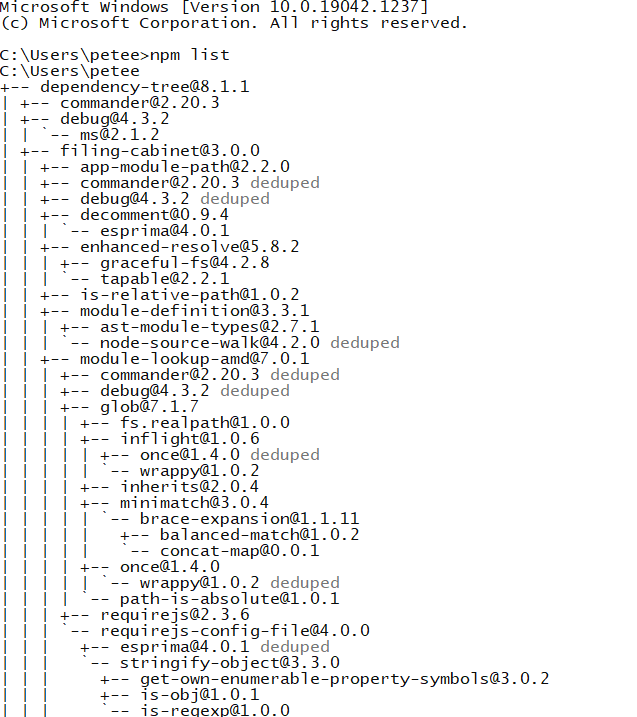
\includegraphics[scale=0.35]{images/npm_ls.png}
		\caption{npm list}
		\label{fig:npm-ls}
	\end{figure}
	
	\subsection{Dependency cruiser}
	
	A \textbf{Dependency cruiser} egy olyan szoftver, amely validálja és vizualizálja az adott csomag függőségeit, a felhasználó által megadott szabályok szerint.\\
	
	\textbf{Miért nem megfelelő}
	\begin{itemize}
		\item A hangsúly a csomagban a csomag függőségeinek validációján van, azaz megvizsgálja, hogy minden adott-e a rendszeren ahhoz, hogy a csomag működni tudjon.
		\item Az npm list-hez hasonlóan ez is csak a rendszeren telepített csomagokkal tud dolgozni, amely szintén leszűkíti a lehetőségeket, hogy mely csomagokat lehet megvizsgálni.
		\item Bár történik gráfkészítés, azonban ez a gráf nagyobb csomagok esetében hatalmas, az ember számára ránézésre szinte semmitmondó, a gráfot .svg kiterjesztésben lokálisan menti, aminek Kliens oldali elérése nehézkes, elemzésre pedig nem szolgáltat adatokat.
	\end{itemize}
	
	\begin{flushright}
		\cite{dep-cruise}
	\end{flushright}
	
	\begin{figure}[h]
		\centering
		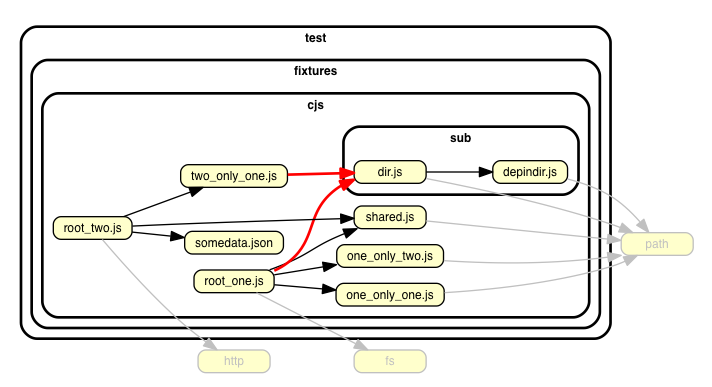
\includegraphics[scale=0.4]{images/dep_cruiser.png}
		\caption{Dependency cruiser}
		\label{fig:dep-cruiser}
	\end{figure}
	
	\subsection{Software Galaxies}
	
	A \textbf{Software Galaxies} egy olyan JavaScript alapú szoftver, amely képes vizualizálni olyan csomagkezelő rendszerek adatait, mint amilyen az npm is. Rendkívül látványos, galaxisra emlékeztető 3 dimenziós objektumot hoz létre, mely a böngészőben jelenik meg és körbejárható. A fejlesztése \textbf{Andrei Kashcha ("anvaka")} nevéhez fűződik.\\
	
	
	\textbf{Miért nem megfelelő}
	\begin{itemize}
		\item Rendkívül nagy a számításigénye. Még erősebb hardveren is érezhető, hogy a 3 dimenziós megjelenítés leterheli a rendszert.
		\item Teljes csomagkezelő rendszereket reprezentál, nem implementálja a csomagok függőségeinek rekurzív keresését, nagy a többletfunkcionalitás az eltérő cél miatt.
		\item Érdekes és látványos (\ref{fig:sw-galaxies} ábra), jól bemutatja a csomagkezelő méretét és nagyságrendjét, amely indokolja hogy ne legyen lokálisan tárolva, azonban ennél többet nem nyújt a feladat szempontjából.
	\end{itemize}
	
	\begin{flushright}
		\cite{anvaka-galaxies}
	\end{flushright}
	
	\begin{figure}[!h]
		\centering
		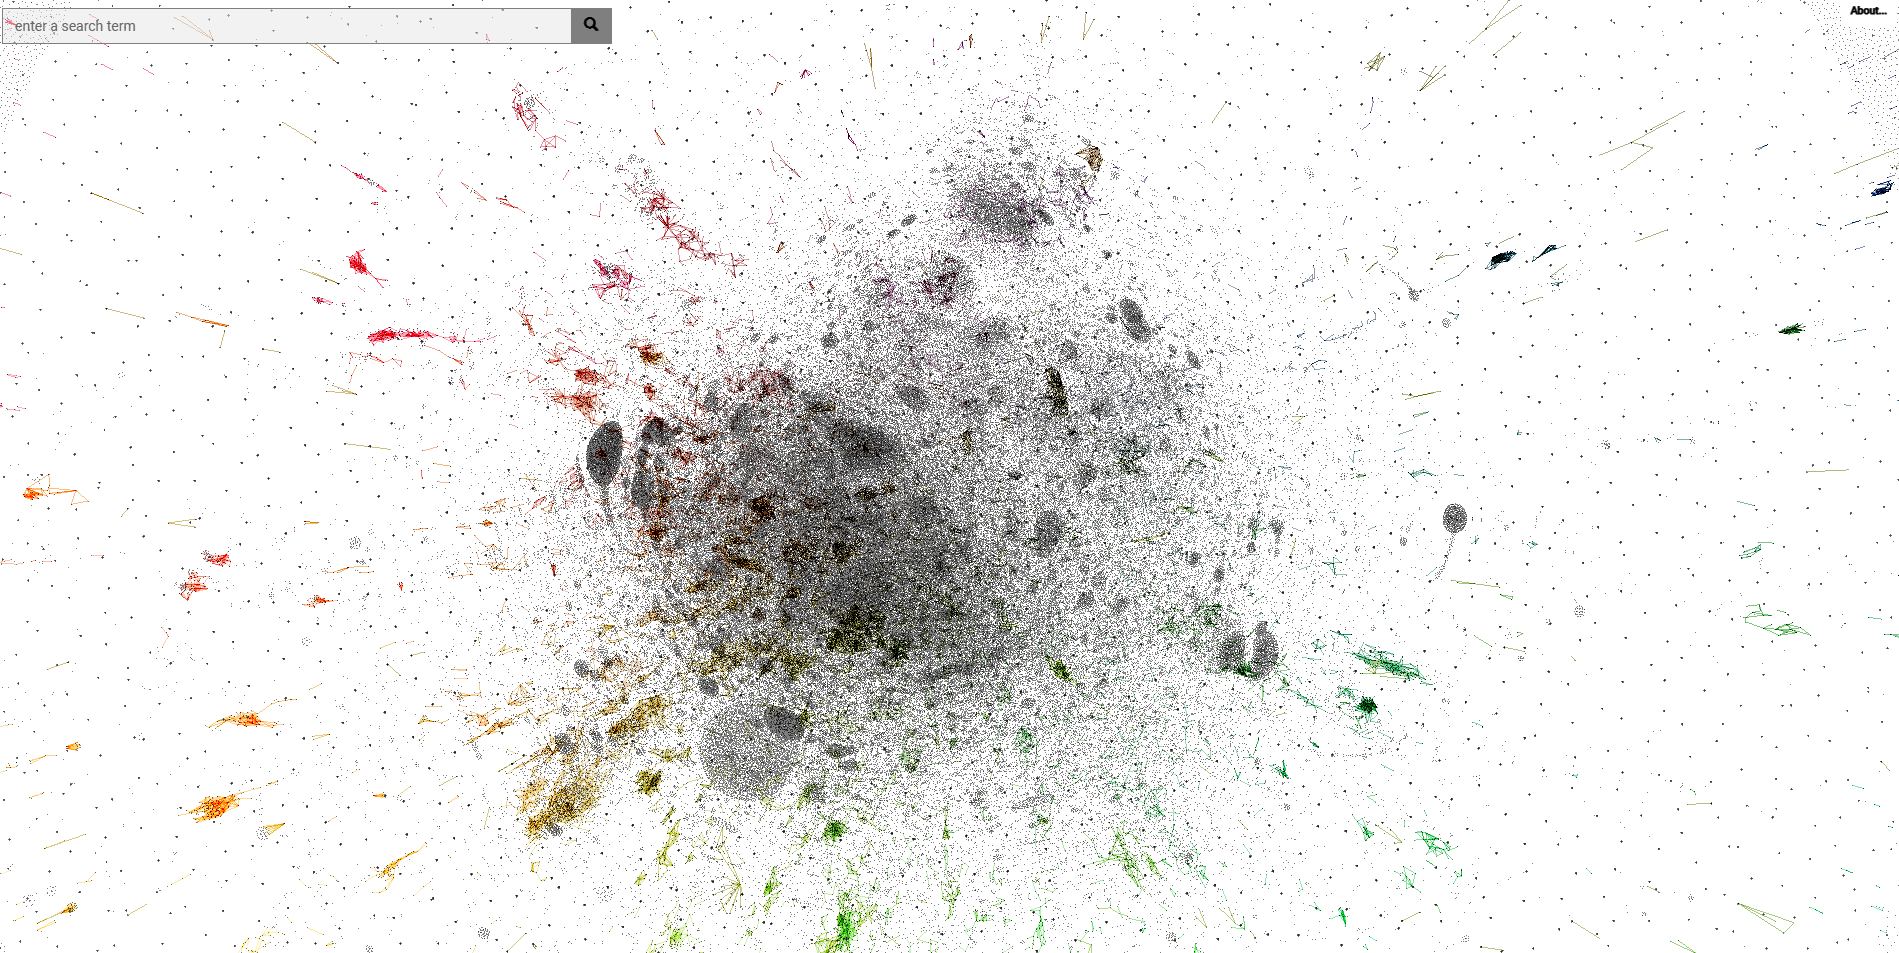
\includegraphics[scale=0.1]{images/anvaka_pm.png}
		\caption{Software Galaxies (Szín invertált)}
		\label{fig:sw-galaxies}
	\end{figure}
	
	\subsection{npmgraph.an}
	
	A \textbf{npmgraph.an} egy olyan JavaScript alapú, Angular.JS keretrendszert használó, interaktív webes szoftver, amely képes vizualizálni egy adott csomag függőségeit gráf formában. A kutatás során ez a szoftver állt a legközelebb az általam tervezett program jellegéhez.	Fejlesztése szintén \textbf{Andrei Kashcha ("anvaka")} nevéhez fűződik.	\\
	
	\textbf{Miért hasznos:}
	\begin{itemize}
		\item A megközelítés hasonló a vízióban felvázolthoz. Azaz kérésekkel, a lokális fájlrendszertől függetlenül szerzi meg rekurzívan a szükséges információt, majd ezeket egy gráfként reprezentálja, verziófüggően.
		\item A program által intézett kérések vizsgálata során kiderült, hogy létezik egy publikus npm registry API, amellyel minden szükséges csomaginformáció lekérhető.
	\end{itemize}
	
	\textbf{Miért nem megfelelő:}
	\begin{itemize}
		\item A vizualizáció hálós gráfként történik, amely nem annyira informatív. A csomagok függőségi gráfja általánosságban egy DAG, azaz irányított, körmentes fagráf, ezt egy hálós gráfos reprezentáció nem használja ki, nem egyértelműsíti sem a mélységet, sem a szinteket és azt sem lehet leolvasni róla, hogy van-e fagráfokra nem jellemző anomália (kör vagy oda-vissza mutató függési viszony).
		\item AngularJS keretrendszert használ, amelyet más, kevésbé fejlett struktúra és funkcionalitás jellemez, mint a jelenlegi Angulart, illetve indokolatlan keretrendszert használni egy ilyen funkcionalitású program kivitelezéséhez.  
	\end{itemize}
	
	\begin{flushright}
		\cite{anvaka-npmgraph}
	\end{flushright}
	
	\begin{figure}[!h]
		\centering
		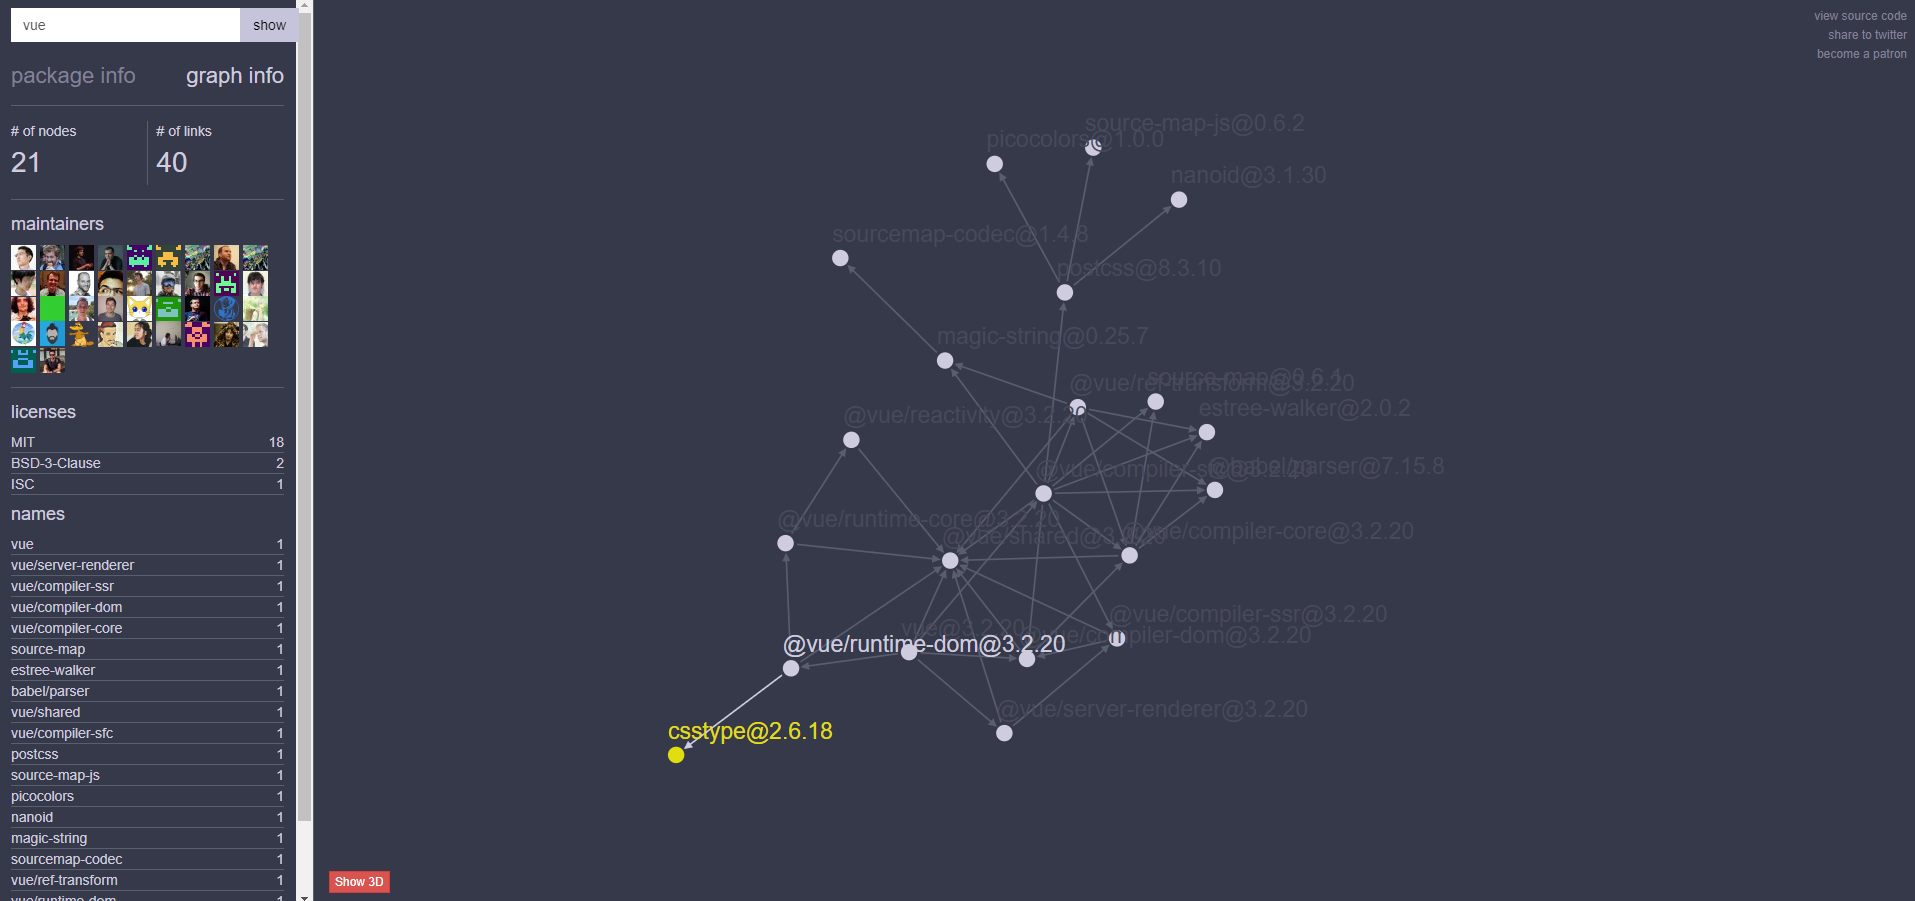
\includegraphics[scale=0.15]{images/anvaka_npmgraph.png}
		\caption{npmgraph.an}
		\label{fig:sw-npmgraph}
	\end{figure}
	
	\pagebreak

\Section{Alkalmazott Technológiák}

A program megtervezésének következő lépése a technológiák, programozási nyelvek kiválasztása, amelyek szükségesek a megvalósításhoz.\\

Mivel a \hyperlink{section.2.2}{vízióban} meghatározásra került, hogy az alkalmazás egy web-applikáció lesz, így ez leszűkíti a kört a webes technológiákra. Mivel a program az adatokat csak feldolgozni fogja, nem pedig tárolni, így sem adatbázis, sem back-end nem szükséges, azaz egy front-end alkalmazás elkészítésére van szükség.\\

A felhasználói interfész lényegében a weboldal felülete lesz, amelynek testreszabása egyértelműen két jelölő nyelvet fog magával vonzani:
\begin{itemize}
	\item HTML5
	\item CSS3
\end{itemize}

A jelölőnyelvekkel szép, áttekinthető UI hozható létre, azonban mivel nem programozási nyelvekről van szó, így szükség lesz egy olyan nyelvre is, amely a kliens oldalon szabályozza a weboldal működését. Webes applikációk esetében leginkább a \textbf{JavaScript}-et szokás használni.\\

\textbf{Hasznos jellemzői:}
\begin{itemize}
	\item Magas-szintű nyelv
	\item Többszörös paradigma támogatás
	\item Futásidejű fordítás
	\item Prototípus alapú objektum orientáltság támogatása
\end{itemize}
\begin{flushright}
	\cite{javascript}
\end{flushright}

A program továbbá a Node.JS-t is alkalmazni fogja, amely a 2. fejezetben bemutatott, aszinkron JavaScript futtatási környezet.

A JavaScript fontos jellemzője az említetteken kívül, hogy egy olyan programozási nyelv, amely az ECMAScript specifikációit követi. A legújabb ECMAScript verzió az ES12 (2021), azonban a legszéleskörűbb támogatást egyelőre az ES6 élvezi a böngészők nagy hányadánál. 

A JavaScript programok strukturálása a korai felhasználási módok miatt egy darabig abszolút nem volt létező fogalom, gyakorlatilag egy \texttt{.js} fájl tartalmazott minden JavaScript kódot, de volt rá precedens, hogy a html kódban a \texttt{<script></script>} tag-ek közé került a kód.

Bár mára a JavaScriptben lehetőség van funkciók, osztályok exportálására és importálására, ezt sokáig csak megkerülni tudták valamilyen más módszerrel.

Az npm-ben nagyon népszerű a \textbf{Babel}, egy olyan JavaScript fordító, amely képes az ES6+ veriójú JavaScript kódok ES5 verziójúra fordítani és futtatni.

A program megfelelő strukturálása, a téma és az esetlegesen hasznos csomagok miatt kényelmes megoldásnak bizonyul a programot egy \textbf{Babelt} alkalmazó \textbf{npm csomagként} megírni, illetve érdekességként a kész program képes lesz önmagát is elemezni.

A program funkcionalitása nem indokolja JavaScript keretrendszer szükségességét.

\pagebreak

\Section{Tervezés}

\subsection{Felhasználói Interfész}

A felhasználói interfész megtervezésénél a fejlesztő szabad kezet kap, azonban célszerű néhány dologra odafigyelni:

\begin{itemize}
	\item Legyen minden egyértelmű
	\item Ne árassza el a felhasználót információval
	\item Maradjon konzisztens
\end{itemize}

\noindent A mai eszközök eltérő méretű kijelzői miatt célszerű az alábbiakra is odafigyelni:

\begin{itemize}
	\item A képernyő méretének változásával ne veszítse el jellegét
	\item Gondosan legyen megtervezve, hogy különböző méretű kijelzők esetén hogy viselkedjen a weboldal
	\item Véletlenül se tűnjön el az információ bizonyos képméreteknél, tehát ne legyen statikus elem
\end{itemize}

Erősen opcionális, azonban érdemes követni a dizájn trendeket, legalább egy alapvető szinten. A program felhasználói felülete ebben az esetben leginkább a "Material UI" dizájnelveit fogja követni, illetve a szemek kímélése érdekében implementálásra kerül majd a lehetőség, hogy a felhasználó váltson sötét és világos mód között.\\

A program felhasználói felületének látványterve alább látható:

\begin{figure}[!h]
	\centering
	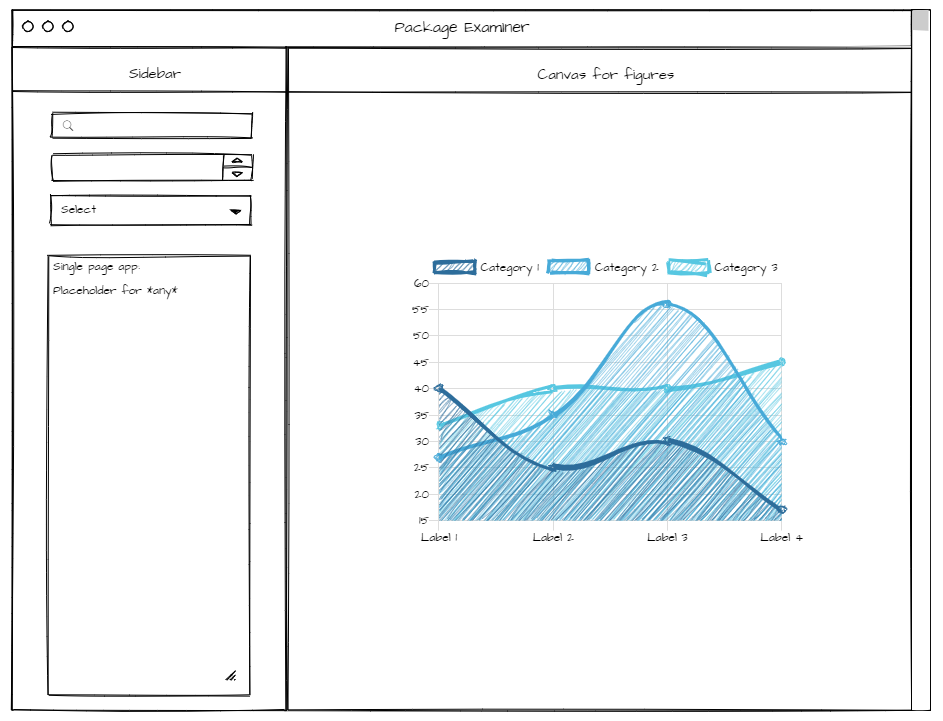
\includegraphics[scale=0.5]{images/ui_plan.png}
	\caption{UI látványterv}
	\label{fig:ui_plan}
\end{figure}

\pagebreak

\subsubsection{UI Látványterv (\ref{fig:ui_plan} ábra)}
\begin{itemize}
	\item A UI két részre lesz felbontva 25-75\% arányban.  A kisebb rész a Sidebar, oldalsó vezérlőpanel lesz, míg a nagyobbik a Canvas, vagyis a "vászon".
	\item A Sidebar-on fog elhelyezkedni minden beviteli mező és gomb, illetve kisebb ábrák, információk kijelzésére lesz alkalmas.
	\item A Canvas lesz a vászon a program számára. Ide fogja kirajzolni a függőségi gráfokat, illetve a nagy méretű diagramokat.
\end{itemize}

\subsection{A Program Szerkezete}

A program egy npm csomagként fog elkészülni, ennek megfelelően szükség lesz az npm \hyperlink{section2.2}{2. fejezetben tárgyalt csomagokra irányuló követelményeinek} az implementálására.\\

\textbf{Az applikáció jellege:}

\begin{itemize}
	\item A weboldal "single-page", azaz egy oldalra tartalmat dinamikusan betöltő web alkalmazás lesz.
	\item Az app szerkezetének és a kód strukturálásának az alapját a tervezett felhasználó interfész elrendezése, és működése fogja adni.
\end{itemize}

\noindent Alapvető építőelemei \textbf{modulok} lesznek, amelyeknek két fajtáját fogja megkülönböztetni:

\begin{itemize}
	\item Template jellegű modulok
	\item Function jellegű modulok
\end{itemize}

\noindent A program alapvetően két módon lesz képes futni:

\begin{itemize}
	\item Egy lokális fejlesztői szerveren, ami reaktív, azaz folyamatosan figyeli a kód változtatásait.
	\item Publikált weboldalként amelyet bármely webszerverről futtatni lehet.
\end{itemize}

\noindent A publikált weboldal esetében a JS keretrendszerektől is megszokott módon a fordítás során egy nagy JavaScript fájl fog készülni, amely az összes JS kódot tartalmazni fogja, így a modulok lényegében csak a fejlesztés átláthatóságában fognak szerepet játszani.

\noindent A tervezett funkcionalitás megvalósításához felhasznált csomagok:
\begin{itemize}
	\item \textbf{Babel}, a már korábban leírt funkciók kivitelezéséhez
	\item \textbf{Parcel}, publikus "build"-be rendszerező csomag
	\item Valamilyen ábrák készítésére alkalmas csomag
\end{itemize}

\noindent A programot felépítő modulok tervezett szerkezetét ábrázolja a \ref{fig:struct_plan} ábra, a következő oldalon.

\begin{figure}[!h]
	\centering
	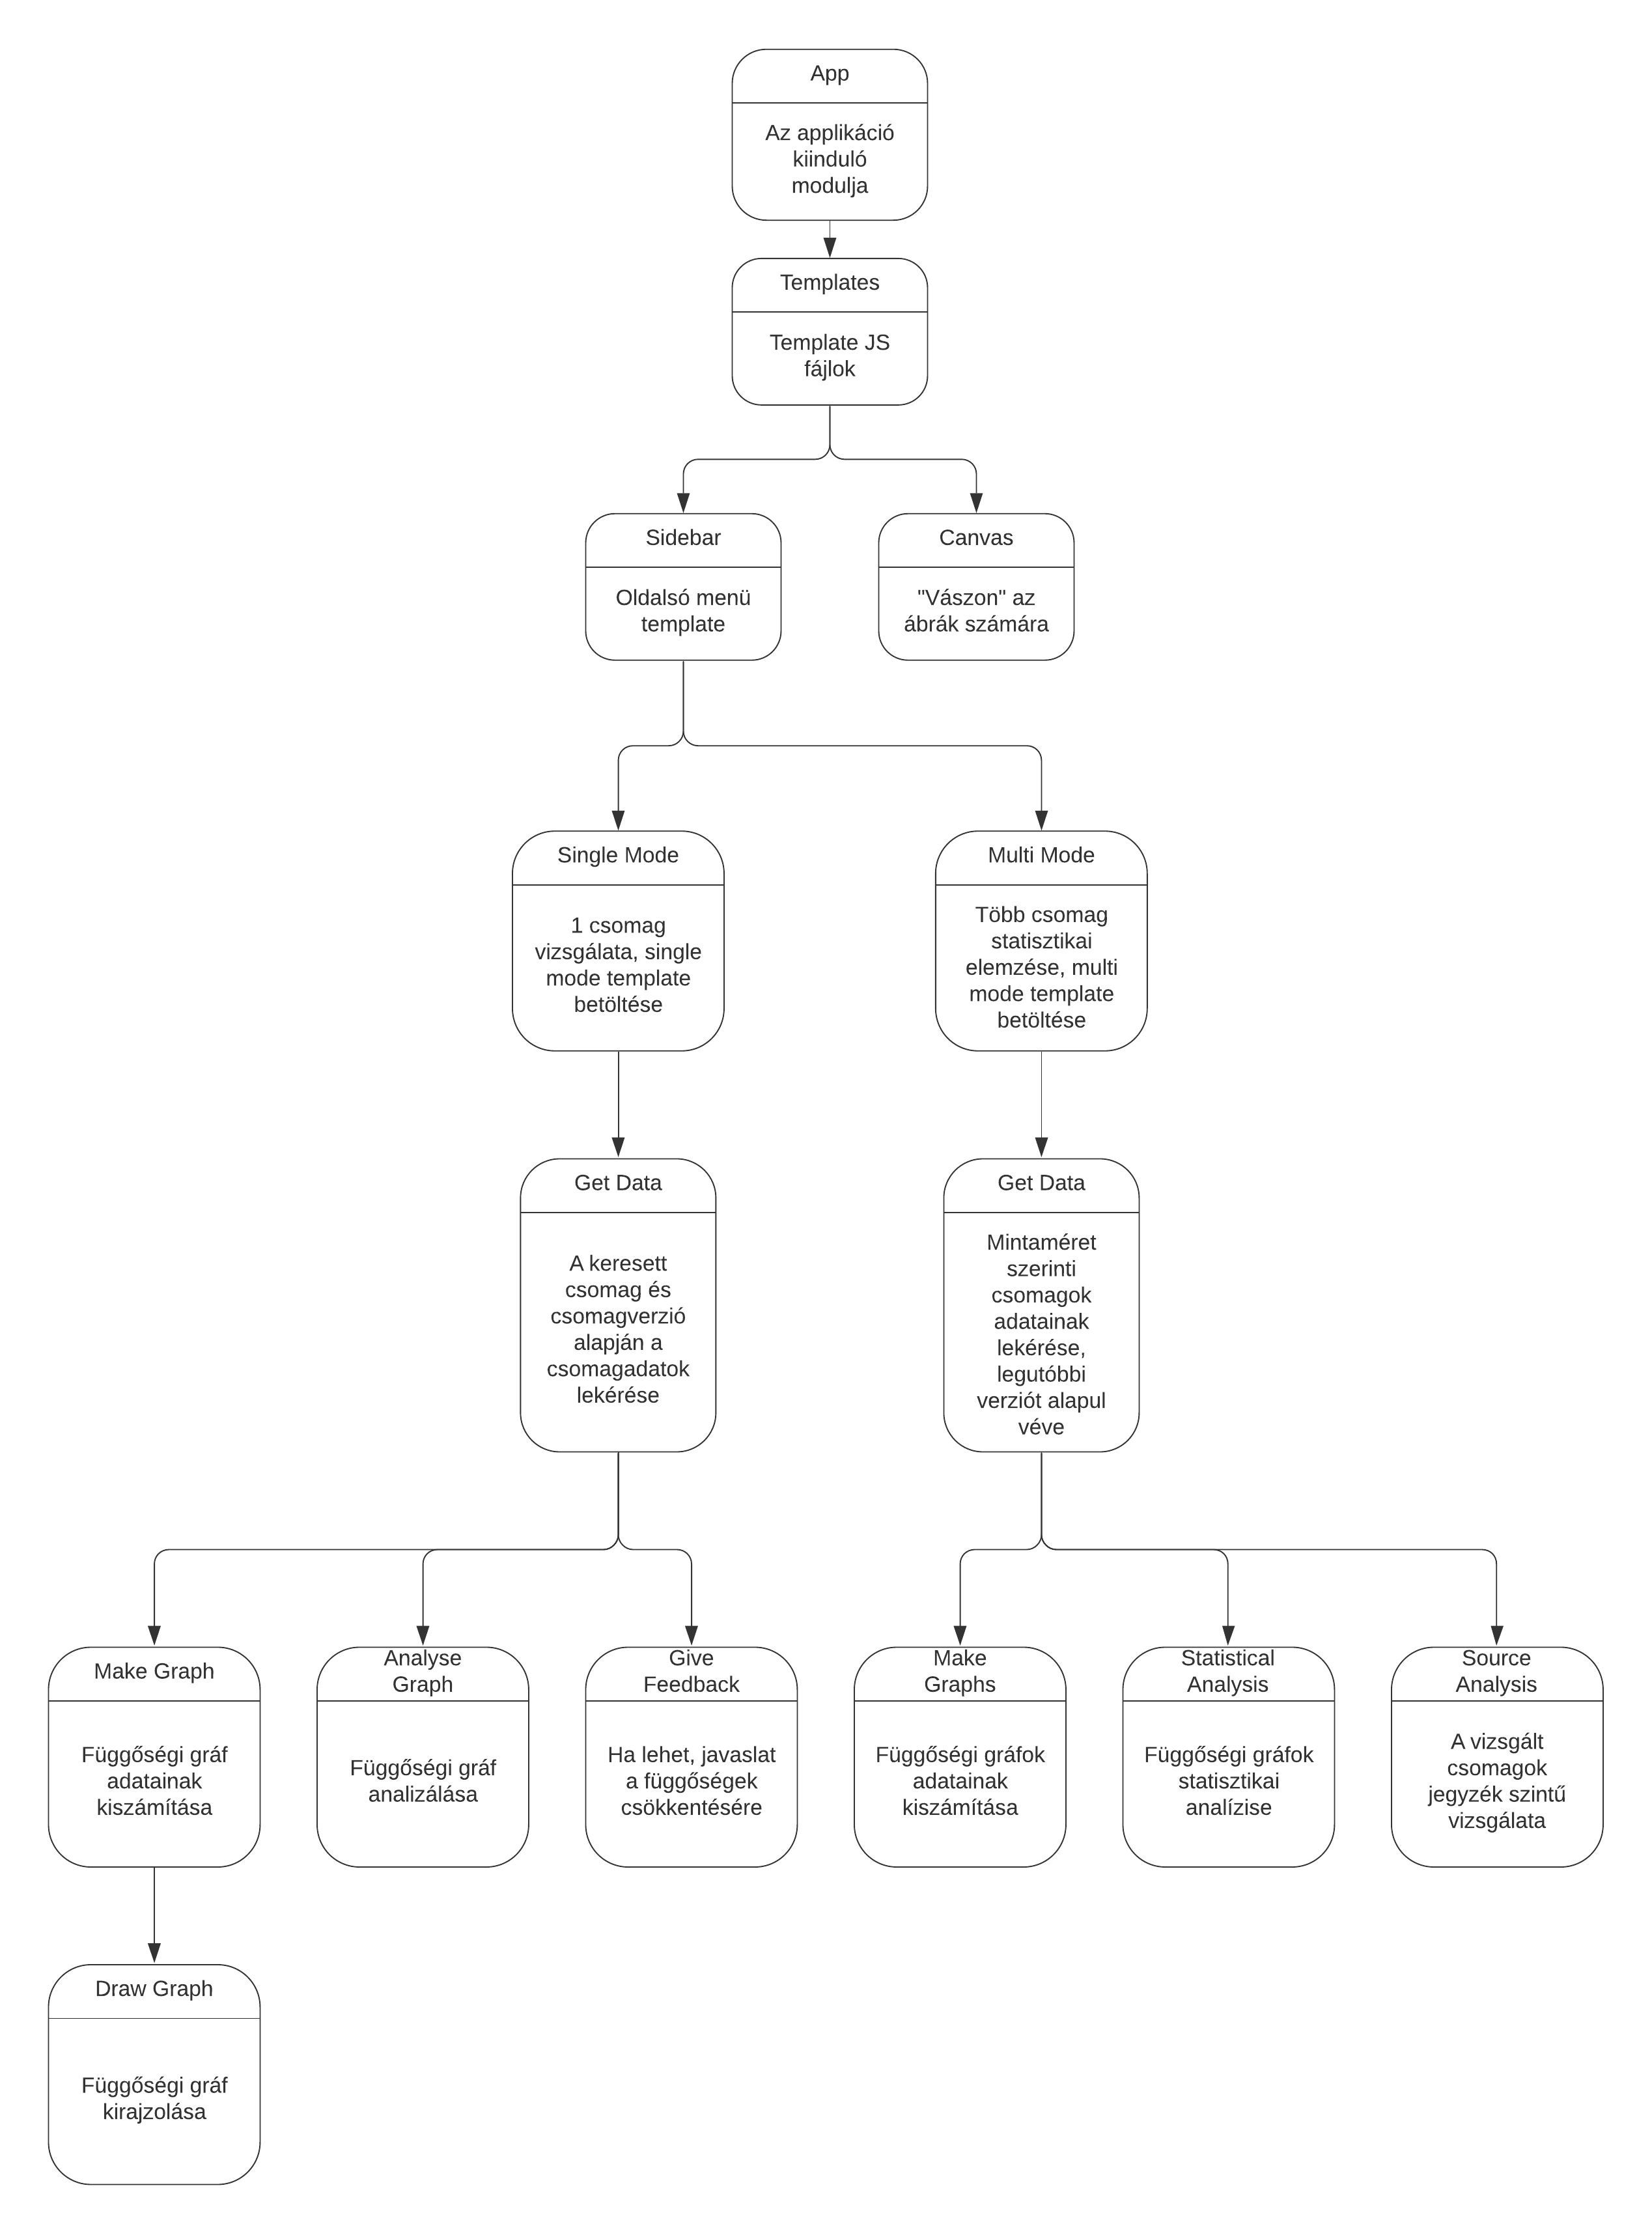
\includegraphics[scale=0.7]{images/struct_plan.png}
	\caption{Szerkezeti terv}
	\label{fig:struct_plan}
\end{figure}


 
